In this chapter, we present one of the main results of this thesis:
the NLO QCD predictions for the production of \Wbb{} in association with up to three light jets.
We carry out the computation in the four-flavor-number scheme (4FNS), thus including effects due to the non-vanishing bottom-quark mass.
The motivation to undertake this challenging computation is two-fold.
Firstly, the class of processes we consider are important irreducible backgrounds to the recently discovered decay of the Higgs boson 
to a pair of bottom quarks, produced in association with heavy vector bosons \cite{Sirunyan:2018kst,Aaboud:2018zhk}.
By providing NLO QCD predictions in samples of light-jet multiplicity we hope to improve the theoretical 
understanding of the backgrounds, and, herewith, improve the measurements of the observables associated to 
the coupling of the Higgs boson to bottom quarks.
Secondly, understanding of one-loop numerical unitarity methods with massive particles
was an important stepping stone towards extending the computational techniques to a multi-loop setting,
and tackling much more complicated two-loop amplitudes in \cref{chap:5parton}.
In particular, the ideas of \cref{chap:dshel} have originally arisen from the necessity of the efficient
numerical evaluation of one-loop helicity amplitudes with external massive quarks.

This work is published in \cite{Anger:2017glm}, 
and the presentation in this chapter follows closely the one from the article.
In \cref{sec:wbb:relevance} we overview the status of theoretical and experimental studies of
the \Wbb{}+jets production, and its phenomenological relevance.
In \cref{sec:BHMassiveImpl} we briefly note on some of the
key developments we have implemented in a new version of the \BlackHat{} library,
which we employed to obtain the virtual matrix elements for this process.
In \cref{sec:wbb:setup} we discuss out computational setup for the Monte-Carlo integration
in \cref{sec:wbb:mc_integration}. Finally, in \cref{sec:wbb:pheno} we present our phenomenological studies.

\section{Introduction}
\label{sec:wbb:relevance}

The first NLO QCD theoretical studies of the \Wbb{} production were carried out in 
the context of the 4FNS in the approximation of massless bottom quarks about 20 years ago \cite{Bern:1997sc,Ellis:1998fv},
and were implemented in the first version of the MCFM program~\cite{mcfm7}.
The first results including the bottom-quark mass, but with on-shell $W$-boson 
appeared in \cite{FebresCordero:2006sj,Cordero:2009kv,Badger:2010mg,Oleari:2011ey}.
The phenomenological studies of NLO QCD \Wbbnj[1]{} production have be performed in \cite{Luisoni:2015mpa}.
Also, related studies of inclusive production of $W$-boson with a single $b$-tagged jet
can be found in \cite{Campbell:2006cu,Campbell:2008hh,Caola:2011pz}.
Finally, the signature of the process \Wbb{}+jets can be also produced from
the off-shell decays of the top quarks, which was studied in \cite{Denner:2017kzu}.
On the experimental side, several dedicated measurements
have been performed by the CDF \cite{Aaltonen:2009qi}, D0 \cite{D0:2012qt}, ATLAS \cite{Aad:2013vka}, and CMS \cite{Chatrchyan:2013uza,CMS:2016bb}
experiments.

In \cite{Anger:2017glm} we presented, for the first time, NLO QCD corrections to \Wbbnj[2]{} and
\Wbbnj[3]{} production. As illustrated in \cref{fig:wbb_channels} for an examples of $n=2$ light jets,
the final state signature we consider can be produced through different orders of the EW and strong couplings.
We study the QCD corrections of to the LO $\order{\alps^{2+n}\alpf^2}$ production,
which are the most important contribution outside of the single or double top-quark resonant regions.
Near the resonances the most important contributions are obtained from the QCD corrections to the LO $\order{\alps^{n}\alpf^4}$ production,
and EW corrections to the LO $\order{\alps^{1+n}\alpf^3}$. The latter were studied in \cite{Denner:2017kzu}.

\begin{figure}[t]
  \centering
  \includegraphics[width=0.8\textwidth]{wbb_channels}
  \caption{
    Different contributions to the $W(\to 2l)b\bar{b}jj$ final state.
    We consider the NLO QCD corrections to the channel with the least power of the EW coupling $\alpha$, which
    is dominant outside of the top-quark resonance region.
    The figure is based on \cite{Denner:2017kzu}.
  }
  \label{fig:wbb_channels}
\end{figure}


Already the firs studies of \Wbb{} production
recognized \cite{Ellis:1998fv,FebresCordero:2006sj,Cordero:2009kv} that the NLO QCD corrections are large. 
The main reasons are that the real radiation opens a new
gluon-induced production channel, and the that
the kinematical constraint on the transverse momentum of  $W$ is released.
These effects are collectively known as ``giant $K$-factors'' \cite{Rubin:2010xp}. 
Including an additional light jet in the final state improves the  behavior \cite{Luisoni:2015mpa}.
However only starting from \Wbbnj[2]{}, i.e.\ from two additional light jets, are all possible production
channels open at the LO.  We show that this in this case, as expected, the $K$-factors are moderate.


One of the first ideas to address the problem of large $K$-factors was exploiting the jet vetoes 
for more exclusive studies \cite{FebresCordero:2006sj}.
Unfortunately, the sensitivity to the $p_T^{\textrm veto}$ cut upsets
the precision  of the predictions in this case.
The latter can be mitigated by employing the so-called ``exclusive-sum'' techniques \cite{ESums},
which take advantage of the available multi-jet NLO samples.
In particular, we use them in \cref{sec:wbb:pheno} for our predictions of observables associated to the  $H(\rightarrow b{\bar b})W$ 
production: the $p_T^{b\bar b}$, $p_T^W$, and $M_{b\bar b}$ distributions.

%%%%%%%%%%%%%%%%%%%%%%%%%%%%%%%%%%%%%%%%%%%%

\section{Numerical Unitarity with Massive Particles in \BlackHat{}}
\label{sec:BHMassiveImpl}

The original version of the \texttt{C++} library \BlackHat{} \cite{Berger:2008sj,Berger:2008ag} has been
implemented having only massless QCD in mind. 
And the technical details went into that implementation are very different than
the multi-loop generalization we presented in \cref{chap:numunitarity}.
In this section we discuss the developments for the new version of \BlackHat{},
which has been required to be able to compute one-loop amplitudes with massive quarks.

A comprehensive review of the issues connected with the application of
one-loop numerical unitarity methods to massive particles can be found in \cite{Ellis:2011cr,Ellis:2008ir}.
Furthermore, some details of our implementation have been already discussed in \cite{FelixDiss},
so we limit ourselves to a very brief summary.

\paragraph{The strategy of handling the dimensional regularization}
was the most significant change.
The \BlackHat{} library was based on the numerical unitarity methods in four dimensions to extract the cut-constructable part
of the amplitude \cite{Ita:2011hi,Berger:2008sj,Berger:2008ag}. As for the rational part, either the special on-shell recursion, or the SUSY decomposition, have been employed.
Both approaches are not suitable for amplitudes with massive quarks.
To this end, we have reorganized the computation strategy to follow closer the $D$-dimensional unitarity method described in \cref{chap:numunitarity}\footnote{
  We did not, however, introduce the $D$-dependence into the coefficients as we did in the examples in \cref{sec:ms_examples}.
},
also taking advantage of our developments in \cref{chap:dshel} with some additional tricks explained in \cite{Anger:2018ove}.

Nevertheless, as an optimization opportunity,
we still extract the cut-constructable coefficients by sampling 
the cut equations \eqref{eq:cut_equations} 
with the four-dimensional loop momenta first.
We then transfer these coefficients to the left-hand side of \cref{eq:cut_equations} and use only a few additional
sample points with five-dimensional loop momenta to obtain the remaining coefficients.
This, in turn, implies that the general parametrization of on-shell loop-momenta, that we discussed in \cref{sec:evaluation_of_cuts},
is not suitable\footnote{
  it is also not suitable for the reason of numerical stability
}. For this reason we have constructed and implemented the on-shell loop-momenta parametrizations
for all topologies with massive particles in the loop, based on \cite{Kilgore:2007qr}.



\paragraph{The extraction of master coefficients} was previously organized according to a more analytics-oriented approach of \cite{Forde2007}.
With massive particles in the loop this approach becomes rather clunky.
Furthermore, we found that it does not offer any benefits over numerically-oriented OPP-like subtractions
in the cut equations \eqref{eq:cut_equations}. Therefore, we replaced the former by the latter.


\paragraph{Additional topologies.}
The tadpole and bubble topologies with the single on-shell particle in the corner (which we dub ``on-shell bubbles'')  no longer correspond to scaleless
integrals if massive particles are involved, hence they cannot be discarded.
We have implemented the construction of hierarchies for these topologies, as well the corresponding
on-shell loop-momentum parametrizations. 
In addition, there are some new features associated to these topologies:
\begin{enumerate}
  \item The cuts of all tadpoles and on-shell bubbles contain explicitly divergent contributions associated
    to the mass and wave-function renormalization (see \cref{fig:wbb:singdoublecut} for an example).
    We mentioned this towards the end of \cref{sec:cut_equations}.
    \begin{figure}[h]
      \[
        \vcenter{\hbox{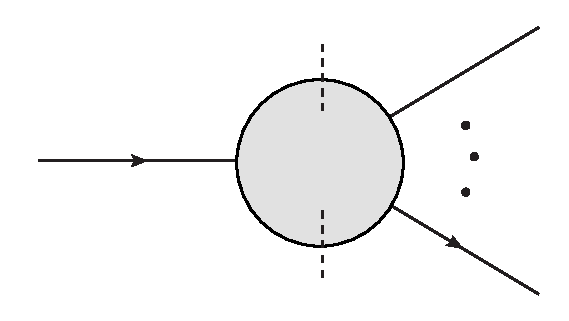
\includegraphics[height=12ex]{./figures/dc_div_left.eps}}} =
        \vcenter{\hbox{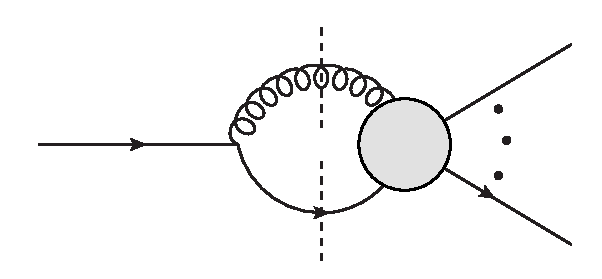
\includegraphics[height=12ex]{./figures/dc_div_r.eps}}}~+~
        \vcenter{\hbox{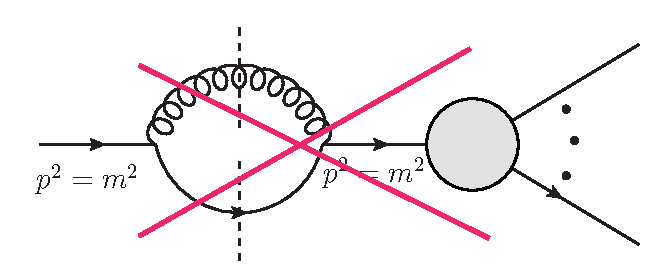
\includegraphics[height=12ex]{./figures/dc_div2_cross.eps}}}
      \]
      \caption{
        A double cut with the single on-shell massive quark in the corner (on the left), containing
        a divergent contribution associated to the mass and wave-function renormalization (the second term on the right),
        which has to be manually removed.
      }
      \label{fig:wbb:singdoublecut}
    \end{figure}
    Following the approach of \cite{Ellis:2008ir} we have implemented the removal of this contributions in our off-shell recursion.

  \item The topology in \cref{fig:dc_div2}, in addition to containing a divergent contribution mentioned above,
    has another special feature: the transverse complement of its single light-like external momentum contains this momentum.
    We discussed this in \cref{sec:ms_examples}.
    \begin{figure}[h]
      \centering
      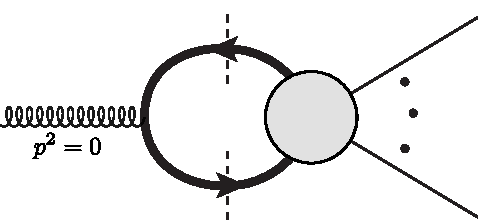
\includegraphics[width=0.3\textwidth]{dc_div2}
      \caption{A special one-loop topology with a massless on-shell leg in the corner and massive cut propagators.}
      \label{fig:dc_div2}
    \end{figure}
    This has two consequences. First, there are more coefficients with master integrals, and we evaluate the corresponding integrals explicitly.
    Second, as opposed to other one-loop topologies, the ansatz for the integrand of this topology is \emph{not} invariant under loop momentum shifts.
    This slightly complicates the construction of hierarchies, since it implies that the tadpoles below have to be carefully aligned.
    Interestingly, this is a generic feature beyond one loop, i.e.\ the ansätze for integrands of \emph{all} topologies are not invariant under loop momenta shifts.
\end{enumerate}


\paragraph{Integrals with internal masses.} Finally,
we have implemented all one-loop master integrals with real internal masses to $\order{\epsilon^0} $, based
on the results from \cite{Carrazza:2016gav,vanHameren:2010cp}. This allows us to incorporate
them in our automated numerical precision tracking and rescue system.

%%%%%%%%%%%%%%%%%%%%%%%%%%%%%%%%%%%%%%%%%%%%

\section{Setup}
\label{sec:wbb:setup}

\subsection{Channels}
\label{sec:calcsetup}

We compute NLO QCD corrections for the production of \Wbb~in association with $n$ light jets ($n =
0,1,2,3$) at the LHC $\sqrt{s} = 13$ TeV. 
We include the leptonic decays of the off-shell vector bosons at the level of amplitudes.
The parton-level cross-sections are obtained from the following channels:
\begin{subequations}
  \begin{align}
    n=0:&\qquad 0\rightarrow Wb{\bar b}q{\bar q}'\ ,\\
    n=1:&\qquad 0\rightarrow Wb{\bar b}q{\bar q}'g\ ,\\
    n=2:&\qquad 0\rightarrow Wb{\bar b}q{\bar q}'gg\ ,\quad  0\rightarrow Wb{\bar b}q{\bar q}'Q{\bar Q}\ ,\\
    n=3:&\qquad 0\rightarrow Wb{\bar b}q{\bar q}'ggg\ ,\quad  0\rightarrow Wb{\bar b}q{\bar q}'Q{\bar Q}g\ ,
  \end{align}
\end{subequations}
which we wrote in a crossing-symmetric form. 
Here the light quarks are denoted with $q$ and $Q$, and the $b$ quarks are considered massive.
The contributions from closed $b$ and $t$ loops are included. \footnote{
  Although the contribution of the latter is negligible.
}
We demonstrate some representative Feynman diagrams contributing to the channels of \Wbbjjj{} in \cref{fig:FDsWbb3j}.

We consider fixed order predictions at parton-level and discard parton-shower
effects. We will require exactly two tagged infrared-safe $b$ jets \cite{Banfi:2006hf}
in all observables we examine.

\begin{figure}[h]
  \centering
  \subfloat[][$qg\rightarrow q^\prime g g W^{\pm}b\bar{b}$]{ 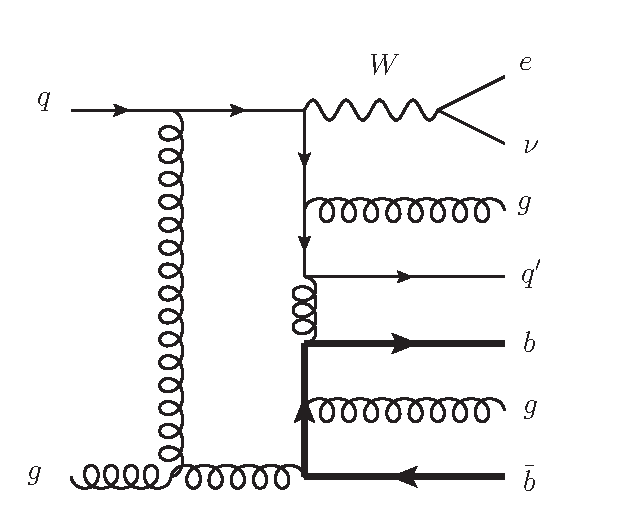
\includegraphics[width=0.28\textwidth]{figures/Wbb2q3g}}
  \qquad
  \subfloat[][$qg\rightarrow q^\prime g g W^{\pm}b\bar{b}$]{\label{subfloat:nf} 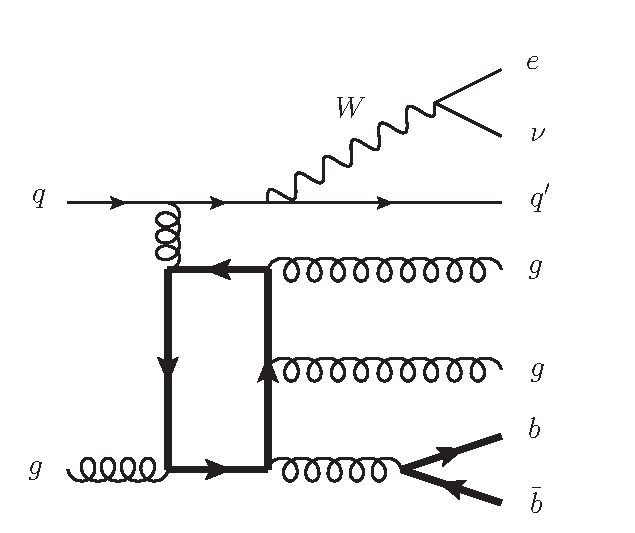
\includegraphics[width=0.28\textwidth]{figures/Wbb2q3g_nf}}
  \quad
  \subfloat[][$q{\bar Q}\rightarrow q^\prime \bar{Q} g W^{\pm}b\bar{b}$]{ 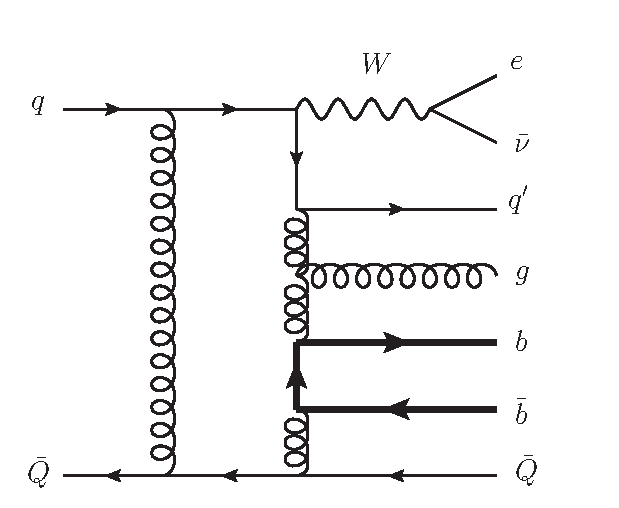
\includegraphics[width=0.28\textwidth]{figures/Wbb4q1g}}
  \caption{Representative one-loop diagrams contributing
    to \mbox{$pp\rightarrow$ \Wbbnj[3]{}} production. Massive quark
    lines are printed thick and the diagram \protect\subref{subfloat:nf} displays a contribution from closed loops of top and bottom quarks.}
  \label{fig:FDsWbb3j}
\end{figure}



\subsection{Renormalization}

We regularize UV and IR divergences in the FDH scheme in the computation of virtual matrix elements,
and use the known transition rules to convert our results to the HV scheme.

\todo{fix error in renormalization}

We give all counter-terms required for the renormalization in the FDH scheme, as well as additional finite shifts in \cref{tab:renorm}.
For the mass and wave-function renormalization we use the on-shell scheme,
and for the $\overline{\text{MS}}$ scheme for the QCD coupling.
\begin{table}[h]
  \begin{tabular}{lcll}
    \textbf{Renormalization} & \textbf{Scheme} & \textbf{Counterterm} \\
    \toprule
    Heavy quark wave function   & on-shell & $\displaystyle \delta_{2,i} ~=~ \frac{N_c^2-1}{2N_c} \left( \frac{3}{\epsilon} + 5 + 3 \ln{\frac{\mu^2}{m_i^2}} \right)$\\
    Light quark wave function   & on-shell & 0\qquad(UV+IR cancellation) \\
    Quark mass            & on-shell & $\displaystyle \delta_{m_i} ~=~ \delta_{2,i}\quad\text{}$\\
    Gluon wave function   & on-shell & $\displaystyle \delta_3 ~=~ \frac{3}{\epsilon} + \sum_i \frac{1}{3}\ln{\frac{\mu^2}{m_i^2}}$\\
    QCD coupling & $\overline{MS}$ & $\displaystyle \delta_{\alps} ~=~ \frac{1}{\epsilon} \left( \frac{11}{3}N_c - \frac{2}{3}(N_f+N_h) \right) - \frac{N_c}{3}$\\
    \midrule
    Decoupling shift & --- & $\displaystyle     \Delta_i ~=~  -\frac{2}{3}\ln{\frac{\mu^2}{m_i^2}} $\\
    \bottomrule
  \end{tabular}
  \caption{The renormalization counter-terms. Here $\mu$ is the renormalization
    scale, $m_{i}$ are the masses for heavy quarks, $N_f$ is the number of light flavors,
    $N_h$ the number of heavy flavors, and $N_c$ the number of colors.
  }
  \label{tab:renorm}
\end{table}
We set $N_f=4$, and $N_h=2$, as we work in the 4FNS, and 
add the decoupling shifts for top and bottom quarks to correctly reproduce the corresponding decoupling limits.
Except for the mass renormalization, which we perform via an explicit computation,
the whole renormalization is proportional to the tree amplitude, 
and the renormalized amplitude $\mathcal{A}^{(ren)}$ is
obtained as
\begin{equation}
  \mathcal{A}^{(ren)} =
  \mathcal{A}^{(bare)}_{m_R} - 4\pi \alpha_s c_\Gamma 
  \left( \sum_i N_{Q_i} \frac{\delta_{2,i}}{2} + N_{g}\delta_3 + \frac{N_{\alps}}{2}\left(\delta_{\alps} + \sum_{i\in N_h}\Delta_i\right) \right)  \mathcal{A}^{(born)},
  \label{renfull}
\end{equation}
where $\mathcal{A}^{(bare)}_{m_R}$ is the amplitude with renormalized masses,
$\displaystyle c_\Gamma={(4\pi)^{-(2-\epsilon)}{\Gamma(1+\epsilon)\Gamma^2(1-\epsilon)}/\Gamma(1-2\epsilon)}$,
$N_g$ and $N_{Q_i}$ are the numbers of external gluons and heavy quarks of flavor $i$ correspondingly,
and $N_{\alps}$ is the power of $\alps$ of the tree amplitude.
We shift \cite{Signer:2008va} the amplitude by
\begin{equation}
  \mathcal{A}^{(ren)}_{HV} - \mathcal{A}^{(ren)}_{FDH} = -4\pi \alpha_s c_\Gamma\left(N_{g}~\frac{N_c}{6} + \frac{N_q}{4}\left(N_c -\frac{1}{N_c}\right)\right)\mathcal{A}^{(born)},
  \label{schemeshift}
\end{equation}
to convert it to the HV scheme.



\subsection{Validation}

The upgrade to the new version of \BlackHat{} involved significant new developments,
as well as replacing a considerable number of old components.
We have extensively validated the new version with the following checks:
\begin{enumerate}
  \item We have reproduced all amplitudes available in \BlackHat{} before the upgrade.
  \item We perform a number of automated internal consistency checks:
    \begin{itemize}
      \item We extend the ansatz for the integrands on the right-hand side of \cref{eq:cut_equations} with the terms which are guaranteed to be zero, for example, by the power-counting constraints.
        We then solve the equations for the coefficients, and check if the coefficients of these term vanish.
      \item We check the known pole structure \cite{Catani:2000ef} of each primitive amplitude.
    \end{itemize}
  \item We have checked the IR poles of squared matrix elements against the integrated subtraction terms,
    as implemented in the \SHERPA{} library.
  \item We have reproduced the helicity amplitudes from \cite{Ellis:2008ir}.
  \item We have performed a systematic comparison of squared matrix elements 
    of all subprocesses of $pp\rightarrow t\bar t+(\leq 2)-$jet, $pp\rightarrow b\bar b+(\leq 2)-$, and
$Wb\bar b+(\leq3)-$ processes against publicly available generators 
\textsc{Recola}~\cite{Actis:2016mpe} and \textsc{OpenLoops}~\cite{Cascioli:2011va} 
(both powered by the \textsc{Collier} library~\cite{Denner:2016kdg}).
\end{enumerate}

\subsection{Numerical Stability}
%
In this section, we explore the numerical stability of the new version of \BlackHat{}.
We compare the normal matrix elements $d\sigma_V^\mathrm{prod}$ with the ones obtained from quadruple-precision evaluations $d\sigma_V^\mathrm{HP}$.\footnote{
  We use the \cite{QD} library for high-precision arithmetics
}

\begin{figure}[h]
  \centering
  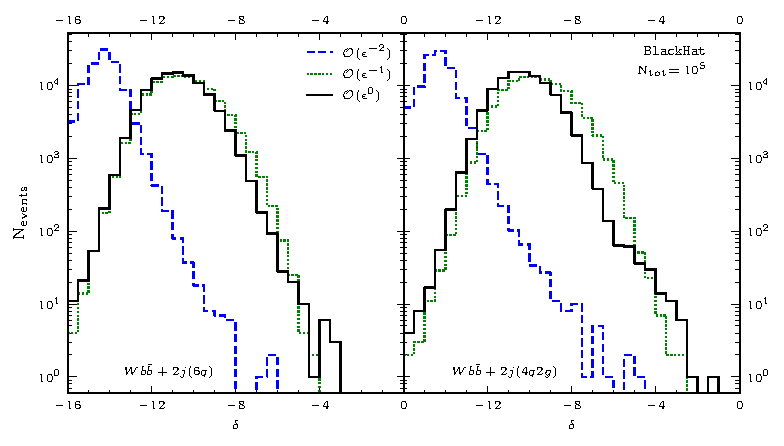
\includegraphics[scale=1.1]{plots/numstab2j}
  \caption{
    The logarithmic relative error of the full-color matrix elements
    for two types of subprocesses contributing to the \Wbbjj~production calculation. On the
    left we show results for the
    six-quark and on the right for four-quark matrix elements, respectively.
    The dashed (blue) line represents the precision of the double pole, the dotted
    (green) line represents the single pole and the
  solid (black) line the precision of the finite piece of the calculation.}
  \label{fig:stabilityWbb2j}
\end{figure}
\begin{figure}[h]
  \centering
  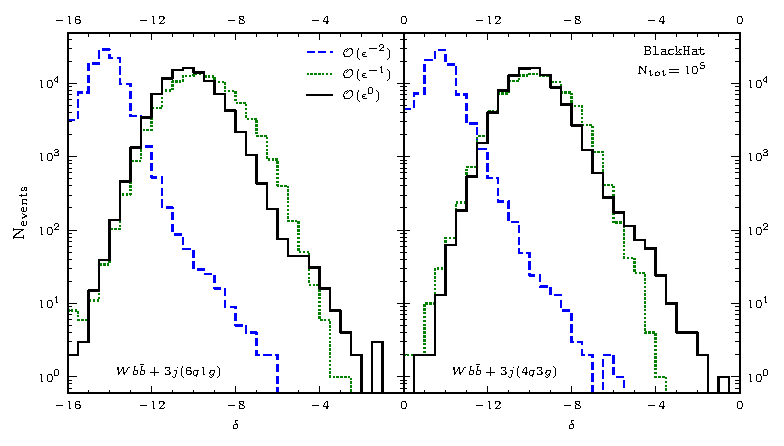
\includegraphics[scale=1.1]{plots/numstab3j}
  \caption{As in \cref{fig:stabilityWbb2j} but for \Wbbjjj{} production,
  considering only the leading-color contributions to the one-loop matrix elements.
  On the left we show results associated to the six-quark and on the right the ones associated to
four-quark matrix elements.}
\label{fig:stabilityWbb3j}
\end{figure}


We study the most complex sub-processes
by generating the histograms (see \cref{fig:stabilityWbb2j,fig:stabilityWbb3j}) of the logarithmic relative error $\delta$,
\begin{equation}
  \delta = \log_{10}\left(\frac{\left|d\sigma^{\text{prod}}_V - d\sigma^{\text{HP}}_V\right|}{\left|d\sigma^{\text{HP}}_V\right|}\right)\ .
  \label{reldiff}
\end{equation}
We sample $10^5$ phase-space points from the same distribution that we used in our phenomenological studies.
Overall we see, that our program is numerically stable,
with only a few points with precision worse then $10^{-3}$,
which have no effect on the observables.

One of the advantages of unitarity methods is that they allow a fine-grained control of the evaluation process.
We convert all the internal consistency tests listed in the previous section into
the precision-monitoring system.  
It identifies when the computation becomes unstable, and reevaluates
only the small part with higher precision whenever required.



\section{Monte Carlo Integration}
\label{sec:wbb:mc_integration}



We employ \SHERPA{}\cite{Sherpa} for managing the Monte-Carlo integration,
subprocess generation and phase-space mappings.
And we interface it to our library for virtual matrix-element generation.
We split the virtual matrix elements into leading and subleading color contributions
to optimize the integration. The latter are more expensive to compute, but contribute less to the observables,
so they can be samples less frequently \cite{BH:W3jDistributions,Ita:2011ar}.
We employ massive dipoles \cite{Catani2002} for IR subtraction as implemented in \COMIX{}~\cite{Comix}.
%

We perform a fixed-order parton-level computation. Non-perturbative effects, such as hadronization, as well as parton showers are considered in our study.
All results that we provide are fixed-order parton-level predictions and we include neither parton-shower effects nor hadronization corrections or other
non-perturbative effects.

\subsection{Input Parameters: Partons Distributions, Couplings and Masses}
\label{sec:base_setup}
We use PDFs from {\texttt CT14}~\cite{CT14},
with LO ({\texttt CT14llo\_NF4}) and NLO ({\texttt CT14nlo\_NF4}) PDF sets, as
implemented in the LHAPDF library~\cite{LHAPDF}. 
The strong coupling is taken to by $\alps(M_Z)=0.125$ at LO and
$\alps(M_Z)=0.1128$ at NLO. 
The bottom-quark mass is $m_b=4.75$ GeV.

The electroweak parameters are evaluated in the LO $G_\mu$ scheme \cite{Denner2000c}. The fixed and computed
parameters as given in \cref{tab:ewinput}. The $\alpf(M_Z)$,
$\sin^2(\theta_W)$ and $g_W^2$ are computed with
\begin{align}\label{eq:ewlorel}
\sin^2(\theta_W) &= \left(1-\frac{M_W^2}{M_Z^2}\right)\ , & \alpf(M_Z)&=\frac{\sqrt{2}}{\pi}G_F M_W^2
  \sin^2(\theta_W)\ ,\notag\\
g_W^2&=\frac{4\pi\alpf(M_Z) }{\sin^2(\theta_W)}\ .
\end{align}

\begin{table}[]
  \centering
  \begin{tabular}{p{3.5cm}p{5cm}}
    \toprule
    Parameter & Value  \\
    \midrule
    $G_F$ & $1.1663787 \times 10^{-5}$ GeV$^{-2}$ \\
    $M_W^{\text{OS}}$& $80.385$ GeV \\
    $M_Z^{\text{OS}}$& $91.1876$ GeV \\
    $\Gamma_W$& $2.085$ GeV \\
    $\alpf(M_Z)$ & $1/132.23$ (calculated)\\
    $\sin^2(\theta_W)$ & $0.22290$ (calculated)\\
    $g_W^2$ & $0.42635$ (calculated)\\
    \bottomrule
  \end{tabular}
  \caption{Electroweak parameters used in our study, which are chosen in accordance with 2016 PDG values~\cite{Patrignani:2016xqp}.}
  \label{tab:ewinput}
\end{table}

The CKM matrix is approximated by a unit matrix. 
The leads to difference of  the order of at most 1\%,
as determined from the LO analysis.

We find that the contribution of the closed top quarks has a order $1\%$ effect on
the cross-sections. This is according to expectations ~\cite{BH:W4j,BH:Z4j,Campbell:2016tcu}. 

\subsection{Kinematics, Observables and Exclusive Sums}
\label{sec:kin}
In this section, we provide the definition for observables we employ in our study.
The pseudorapidity $\eta$ and the
angular separation between two partons, leptons, or jets $\Delta R$ are defined as
\begin{align}
  \eta &= -\ln\left(\tan\frac{\theta}{2}\right),&  \Delta R &= \sqrt{(\Delta \phi)^2+(\Delta \eta)^2}.
\end{align}
Here $\Delta\phi$ is the difference in the azimuthal angle in the transverse plane,
$\theta$ is the polar angle with respect to the beam axis, and
$\Delta\eta$ the difference in $\eta$. 
The transverse energy of $W$, $E_T^W$, and the total partonic transverse energy $\HTpartonicp$ are defined as
\begin{align}\label{eq:htpart}
  E_T^W&=\sqrt{M_W^2+\left(p_T^W \right)^2},& \HTpartonicp&=\sum_j p_{\textrm T}^j+E_{\textrm T}^W, \qquad p_T=\sqrt{p_x^2+p_y^2}
\end{align}
with the sum over all final state partons $j$.
The jet invariant masses are defined by
\begin{align}
  M_{ij}^2 = \left(p_i^{\text{jet}}+p_j^{\text{jet}}\right)^2,
\end{align}
and we label  jets in order of decreasing transverse momentum $p_T$. 
The transverse mass of $W$ is
\begin{align}
  M_T^W=\sqrt{2E_T^eE_T^\nu(1-\cos(\Delta\phi_{e\nu}))}\ .
\end{align}

We now explain how do we build the exclusive-sum observables from multi-jet samples.
We choose the cut $p_{T}^{\text{excl}}$, with respect to which we take an exclusive cross-section $\sigma^{\text{exc}}_n$
for each jet multiplicity $n$, except the one with maximal  $n$, for which we take the inclusive result,
\begin{align}\label{eq:excsums}
  \sigma^{\text{NLO+}}_0 &= \sigma^{\text{exc}}_0 + \sigma^{\text{inc}}_1\ , &
\sigma^{\text{NLO++}}_0 &= \sigma^{\text{exc}}_0 +\sigma^{\text{exc}}_1+
\sigma^{\text{inc}}_2\ .
\end{align}
The expectation is that replacing the, effectively leading order contributions, from the real radiation with the full NLO
corrections mitigates the problem of large $K$ factors, and at the time, the sensitivity to $p_{T}^{\text{excl}}$ is not as high 
as in the case of the exclusive computation.

\section{Phenomenology}
\label{sec:wbb:pheno}
In this section we present NLO QCD results for \Wbbn~production in
$pp$ collisions at $\sqrt{s}=13$ TeV, the experimental configuration
of the LHC Run-II. We present results for a set of distributions and
apply the following cuts
\begin{align}
  p_T^{\text{jet}}&>25\text{ GeV},& |\eta^{\text{jet}}|&<2.4\ ,\notag\\
  p_T^{e}&>25\text{ GeV},& |\eta^{e}|&<2.5\ ,\notag\\
  p_T^{\nu}&>20\text{ GeV},& M_T^W &> 20\text{ GeV}\ .
  \label{eq:Cuts}
\end{align}
The cuts are applied to both light  and
$b$ jets. The renormalization and factorization scales are chosen to be equal and set on an
event-by-event basis by $\mu=\HTpartonicp/2$, according to
\cref{eq:htpart}. We define our jets by employing the
anti-$k_T$ jet algorithm~\cite{antikT} with $R=0.4$, as implemented in the
\texttt{FastJet} package~\cite{Cacciari:2011ma}.

\subsection{Total Cross Section and Scale Dependence}
\label{totalxsw}
In \cref{tab_Wpj_total_xs}, we present total partonic cross sections,
employing the kinematical cuts of \cref{eq:Cuts}, for inclusive production of
both $W^-$ and $W^+$ accompanied by two $b$ jets and zero to three
light jets. The numerical integration uncertainty is given in parenthesis and
the scale dependence is quoted in superscripts and subscripts. We also show
the ratio of NLO over LO results, so called $K$-factors, in separate columns.

We employ the standard dynamical choice of factorization and renormalization scales $\mu_R=\mu_F=\mu_0=\HTpartonicp/2$ (see \cref{eq:htpart}).
We estimate the error from the missing orders of the perturbation series expansion in the coupling constants with the standard technique of
the scale variations around the central scale $\mu_0$. 



%%%%%%%%%%%%%%%%%%%%%%%%%%%%%%%%%%%%%%%%%%%%%% 
\begin{table}[ht]
  \begin{center}
    \begin{adjustbox}{width=1\linewidth}
      \begin{tabular}{ccccccc}
        \toprule
        jets  & \Wbbm~LO & \Wbbm~NLO & $K$-factor & \Wbbp~LO & \Wbbp~NLO & $K$-factor\\
        \midrule
        0  & $0.33278(12)^{+0.0619}_{-0.0490}$ & $0.67719(60)^{+0.1288}_{-0.1000}$  & $2.03$ & $0.48573(19)^{+0.0925}_{-0.0727}$ & $0.97175(85)^{+0.1877}_{-0.1411}$  & $2.00$\\
        1  & $0.36153(13)^{+0.1408}_{-0.0945}$ & $0.50484(63)^{+0.0851}_{-0.0800}$  & $1.40$ & $0.52095(23)^{+0.2034}_{-0.1362}$ & $0.72740(99)^{+0.1277}_{-0.1167}$  & $1.40$\\
        2 & $0.18501(44)^{+0.1053}_{-0.0626}$ & $0.22604(87)^{+0.0407}_{-0.0400}$  & $1.22$ & $0.27663(68)^{+0.1569}_{-0.0934}$ & $0.3340(17)^{+0.0599}_{-0.0647}$  & $1.21$\\
        3  & $0.07204(25)^{+0.0540}_{-0.0289}$ & $0.08288(89)^{+0.0189}_{-0.0200}$  & $1.15$ & $0.11493(59)^{+0.0855}_{-0.0459}$ & $0.1286(17)^{+0.0280}_{-0.0307}$  & $1.12$\\
        \bottomrule
      \end{tabular}
    \end{adjustbox}
     %%%%%%%%%%% TABLE xs  %%%%%%%%%%%%%%%%%%%%%%%%%%
  \end{center}
  \caption{LO and NLO QCD results for inclusive \Wbbpm+$0,1,2,3$-jet cross
    sections (in $pb$). Results with dynamical scale $\HTpartonicp/2$ are shown
    together with their respective $K$-factors.  The setup employed is specified in
    section~\ref{sec:kin}, and kinematical cuts in \cref{eq:Cuts}. Scale
    dependence is shown in superscripts and subscripts. The number in parenthesis next to
    the central value gives the corresponding statistical integration
    error.\label{tab_Wpj_total_xs} }
  \end{table}


%%%%%%%%%%% TABLE ratios  %%%%%%%%%%%%%%%%%%%%%%%%%%
  \begin{table}[ht]
    \small
    \begin{center}
      \begin{adjustbox}{width=1\linewidth}
        \begin{tabular}{ccccccc}
          \toprule
          \multicolumn{1}{c}{ } & \multicolumn{2}{c}{\Wbbp~$n$/\Wbbm~$n$} &
          \multicolumn{2}{c}{\Wbbm~$n/(n-1)$}  &
          \multicolumn{2}{c}{\Wbbp~$n/(n-1)$} \\
          $\qquad n\qquad$ & LO & NLO & LO & NLO  & LO & NLO  \\
          \midrule
          0 &  $1.45962(78)$ & $1.4350(18)$ & --- &  --- & ---  & --- \\
          1&  $1.44098(83)$ & $1.4409(27)$ & $1.08640(55)$ &$ 0.7455(17)$ &$ 1.07253(64)$ & $ 0.7485(12)$ \\
          2&  $1.4952(51)$ & $1.4776(95)$ & $0.5117(12)$ &$ 0.4478(21)$ &$ 0.5310(13)$ & $ 0.4592(24)$ \\
          3&  $1.5952(99)$ & $1.551(27)$ & $0.3894(16)$ &$ 0.3667(44)$ &$ 0.4155(24)$ & $ 0.3850(54)$ \\
          \bottomrule
        \end{tabular}
      \end{adjustbox}
     %%%%%%%%%%% TABLE xs  %%%%%%%%%%%%%%%%%%%%%%%%%%
    \end{center}
    \caption{LO and NLO QCD cross section ratios. The second and third columns
      give charge ratios for both LO and NLO cross sections as a function of the number of
      associated light jets $n$. The last four columns give jet
      production ratios for both \Wbbm~as well as \Wbbp~in association with $n$ light
      jets. These ratios are taken for the cross section of a given
      process to that with one less jet. The number in parenthesis gives the corresponding statistical integration error.\label{tab_xs_ratios} }
    \end{table}
%%%%%%%%%%% TABLE ratios  %%%%%%%%%%%%%%%%%%%%%%%%%%




LO cross sections display a large scale sensitivity, reaching up to 60\% for
\Wbbjjj{} production. We note that the scale dependence of the LO cross section
for \Wbb{} is around $20\%$ while the NLO QCD corrections increase the
total cross section by a factor of 2. This clearly highlights that scale
dependence is in general not representative of the associated theoretical
uncertainties. In this case, the large quantum corrections can be understood as a
result of the opening of gluon-initiated
channels~\cite{Ellis:1998fv,FebresCordero:2006sj,Cordero:2009kv}. Also for \Wbbj{} a gluon-gluon initiated channel is opened
up, but with milder impact, and for the larger multiplicity processes all
subprocesses are present at LO. Hence, quantum corrections are milder
for these processes. Furthermore, kinematical
constraints at LO are only present for \Wbb{} production, as we will discuss for example for the $p_T^{b\bar b}$ and
$p_T^W$ observables in \cref{sec:hw}. As a consequence, we expect quantum corrections for
processes with even more light jets to be under relatively good pertubative control.


In \cref{tab_xs_ratios} we show first, in columns 2 and 3, $W^+/W^-$ charge
ratios as a function of the number of jets. These ratios show a large stability
with respect to the quantum corrections, which have been explored in similar
processes as a way to make precise determinations of ratios of $u/d$ PDFs (see
for example ref.~\cite{Kom:2010mv}). They also show some stability as a function
of the number of jets, with a slight monotonic increase given the larger mean
values of Bjorken $x$ sampled as a consequence of the larger invariant mass necessary to
produce the corresponding final states.

Finally we also explore in \cref{tab_xs_ratios} the jet ratios in $W^\pm
b\bar b$ production in association with light jets. Similarly to studies of these ratios in $W+n$-jet (light jet)
production~\cite{BH:Wratios}, we observe that the results for $n=1$ are special
given the large NLO corrections for \Wbb{} production. The opening of an
initial-state channel makes the
\Wbbj{}$/$\Wbb{} ratio clearly sensible to quantum corrections. In the light jet
study~\cite{BH:Wratios} this was the case for the ratio ($W+2$-jet$)/$($W+1-$jet),
and a full study of jet-ratio universality needed the completion of the NLO QCD
correction to $W+5$-jet production~\cite{BH:W5j}. Similarly, in \Wbb{} inclusive
production, it might be interesting to explore the NLO QCD corrections to
$W+b\bar b+4$-jet production in the future.

In \cref{fig_Wjets_sdep} we study the dependence of total cross sections in
\Wbbm{} and \Wbbp{} production in association with up to 3 light jets on the
renormalization and factorization scale. We employ the central dynamical scale
$\mu_0=\mu_\mathrm{R}=\mu_\mathrm{F}=\HTpartonicp/2$. The scale variations
observed for $W^+$ and for $W^-$ are very similar. The LO cross sections have a monotonically increasing
scale dependence, for $n\geq 1$.  As we observed in the previous subsection, the
scale dependence of \Wbb{} production is special.


%scale dependence for Wm
%%%%%%%%%%%%% FIGURE %%%%%%%%%%%%%%%%%%
\begin{figure}[ht]
\begin{center}
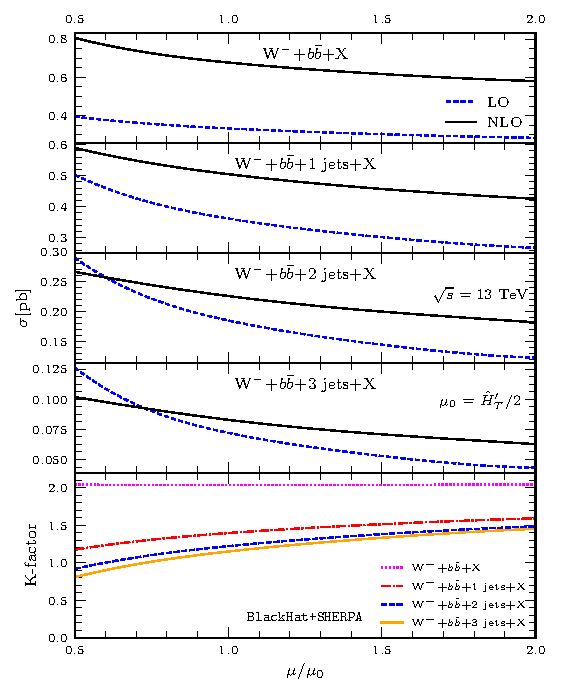
\includegraphics[clip,scale=0.71]{plots/scale_dependence_Wmbb}
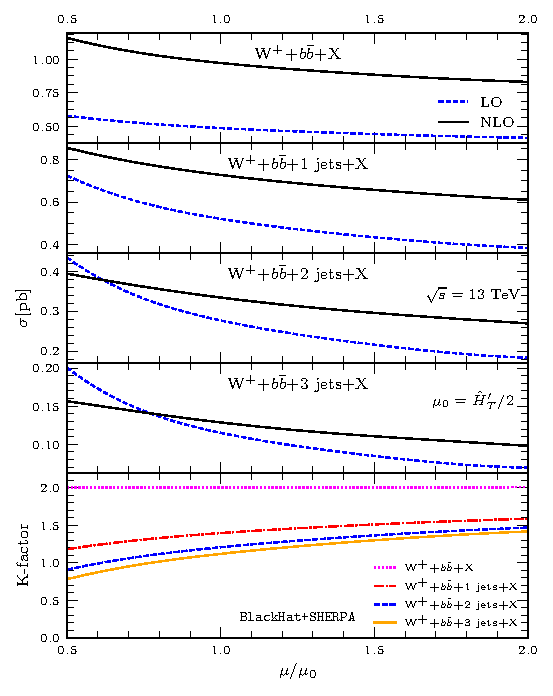
\includegraphics[clip,scale=0.71]{plots/scale_dependence_Wpbb}
\end{center}
\caption{The renormalization- and factorization-scale dependence of total cross
  sections for \Wbbm$+0,1,2,3$-jet$+X$ production in the left and
\Wbbp$+0,1,2,3$-jet$+X$ production to the right,
 with $\mu_0=\mu_\mathrm{r}=\mu_\mathrm{f}=\HTpartonicp/2$. 
The upper four panels show the dependence of LO (dashed blue line) and
  NLO (solid black line) predictions. The lower panel shows
  the K-factor (ratio of NLO/LO).}
\label{fig_Wjets_sdep}
\end{figure}
%%%%%%%%%%%%%%%%%%%%%%%%%%%%%%%%%%%%%%%

We choose the dynamical scale $\HTpartonicp/2$ which on average increases monotonically with multiplicity. For vector boson production in association with massless jets this scale choice
has been observed to produce stable NLO results over a wide range of kinematical
configurations relevant to the LHC and future
colliders~\cite{BH:W3jPRL,BH:W4j,BH:W5j,Mangano:2016jyj}. For the LHC in
particular, it has been observed that for massless jet production the scale
$\HTpartonicp/2$ typically produced NLO cross sections lying on the locus of the
scale-dependence curves. Here we observe that for \Wbbn{} production, the
NLO cross section at the central scale appears consistently on the right of the
scale-dependence plateau. We can assert, in particular considering the
similarities of the massive and massless results studied in
section~\ref{sec:bmass}, that this difference has little to do with the presence
of a massive jet, and it is actually due to the dominant type of subprocess. For
light-jet production those are the ones with a single quark line, while in
the case of \Wbbn{} production the dominant subprocess are those with
two quark lines (those are the subprocesses with most gluons allowed).

Another interesting difference between $W$ production in association with light
jets and \Wbb{} production with multiple light jets, is that for the
former the leading-color approximation for one-loop matrix elements gave a very good
approximation for physical observables (at the level of 1 to
3\%). Contrary to that, \Wbb{} production with light jets is largely dominated by virtual
contributions in our setup, and so the leading-color approximation is at the
order of 10\% for physical observables. That is why all of our results in this
article include full-color information, and we only
exploit the decomposition in a color expansion for efficiency of the
computation. We again attribute this difference to the unlike dominant
subprocesses.


\subsection{Differential distributions}
\label{diffxsw}

In this section, we describe NLO results for several differential
distributions and thereby analyze the impact
that quantum corrections have on fixed-order predictions over phase
space. We generally show results only for one of the $W^\pm$ charges, as the
structure of the corrections are similar between them. 

%pt leading bjet
%%%%%%%%%%%%% FIGURE %%%%%%%%%%%%%%%%%%
\begin{figure}[ht]
  \centering
  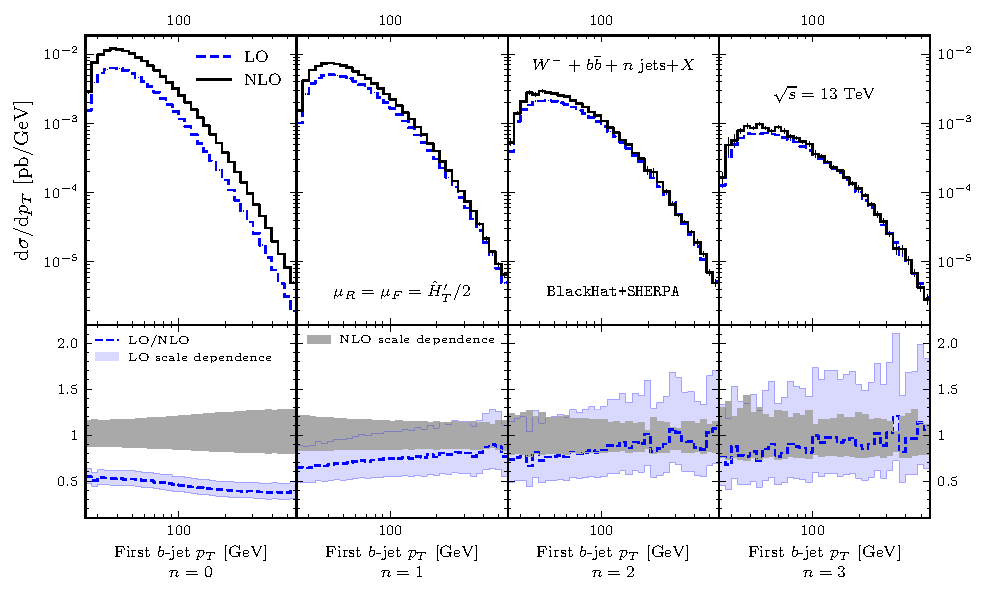
\includegraphics[clip,scale=1]{plots/ptleading}
  \caption{The $\pT$ distributions of the leading $b$ jet (ordered by $p_T$) in inclusive \Wbbm$+n$-jet
    production at the LHC with $\sqrt{s}=13$~TeV. The light-jet multiplicity 
    increases from $n=0$ to $n=3$ from left to right. In the upper panels the
    dashed (blue) lines show the LO results and the solid (black) lines the NLO
    results. Vertical thin lines show the statistical error from the numerical
    integration. In the bottom panels we show the scale-dependence bands
  normalized to the NLO result, in blue for LO and dark gray for NLO.}
  \label{fig_Wmnjpt}
\end{figure}
%%%%%%%%%%%%%%%%%%%%%%%%%%%%%%%%%%%%%%%

%pt subleading bjet
%%%%%%%%%%%%% FIGURE %%%%%%%%%%%%%%%%%%
\begin{figure}[ht]
  \centering
  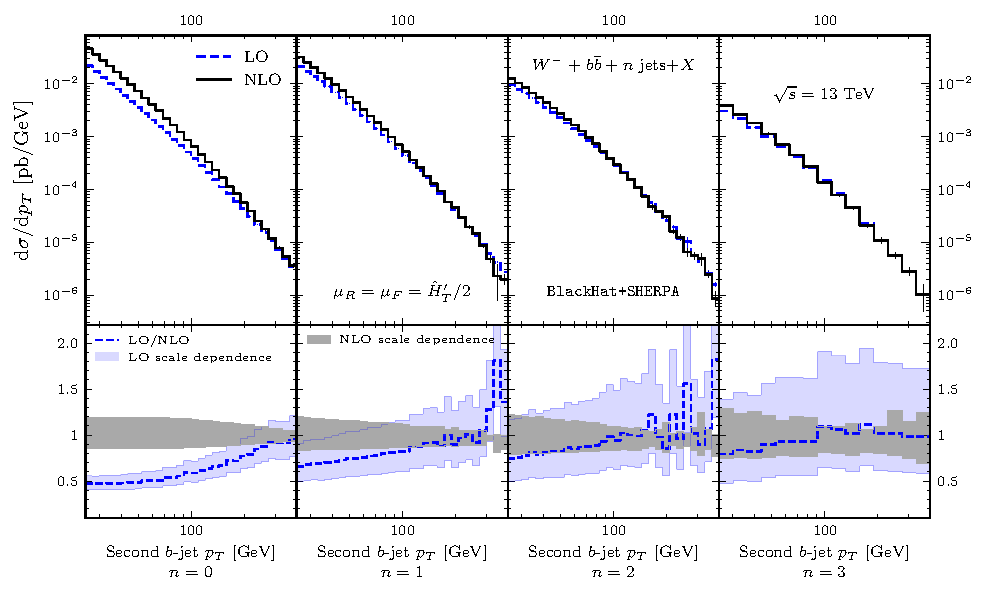
\includegraphics[clip,scale=1]{plots/ptsubleading}
  \caption{The $\pT$ distributions of the subleading $b$ jet (ordered by $p_T$) in inclusive \Wbbm$+n$-jet
    production at the LHC with $\sqrt{s}=13$~TeV. Format as in \cref{fig_Wmnjpt}.}
    \label{fig_Wmnjpt2}
  \end{figure}
%%%%%%%%%%%%%%%%%%%%%%%%%%%%%%%%%%%%%%%

In \cref{fig_Wmnjpt,fig_Wmnjpt2} we show the jet-$p_T$ spectra of the leading
and subleading $b$ jets (ordered by $p_T$) respectively, for inclusive
\Wbbm{} production in association with $n=0,1,2,3$ jets. The upper panel
of the
figures show the LO and NLO distributions in dashed (blue) and solid (black)
lines respectively, while the bottom panels show the scale-dependence bands
normalized to the central NLO result (LO in blue and NLO in gray). Numerical
integration errors for each bin are shown as thin vertical lines (when visible).
All distributions will be shown in a similar manner.

The NLO corrections show quite some structure beyond the $K$-factors studied at
the level of the total cross sections in the previous subsection. We
observe shape differences in most of the $p_T$ distributions of the $b$ jets, in a way
that make the LO predictions usually harder (with the exception of the leading
$b$ jet $p_T$ in \Wbb{} production). Nevertheless, the LO/NLO shape difference
is clearly reduced for the process with highest multiplicity, \Wbbjjj{} production, a
feature that shows up persistently in the following observables.
We notice that the scale dependence of the NLO
results is reduced compared to the LO results (apart from \Wbb{}, as
discussed for total cross sections). In the high multiplicity samples, the NLO results
lie inside the LO bands. 

%Softest light-jet PT
%%%%%%%%%%%%% FIGURE %%%%%%%%%%%%%%%%%%
\begin{figure}[ht]
  \centering
  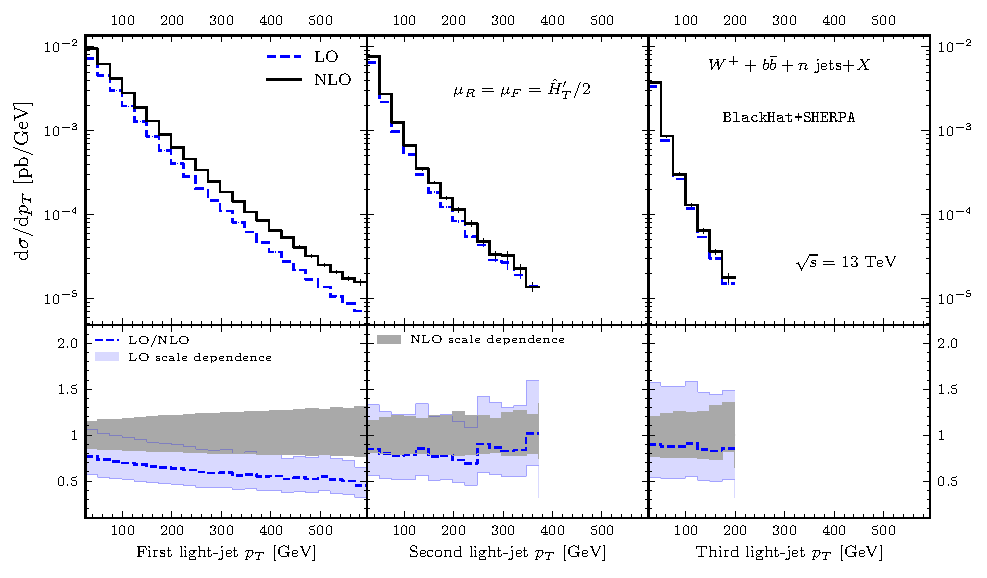
\includegraphics[clip,scale=1]{plots/softestpt}
  \caption{The $\pT$
    distributions of the softest light jet in inclusive \Wbbp$+n$-jet production.
    Format as in \cref{fig_Wmnjpt}.}
    \label{fig_Wmnjptlight}
  \end{figure}
%%%%%%%%%%%%%%%%%%%%%%%%%%%%%%%%%%%%%%%

In \cref{fig_Wmnjptlight} we show the $p_T$ distributions of the softest light jet in
inclusive \Wbbp{}$+1,2,3$-jet production. We observe a considerable reduction of the scale
sensitivity with the inclusion of the QCD corrections, with overlap of the LO
and NLO bands. It is important to note that for these distributions, which are
experimentally very relevant as they are quite sensitive to the jet-energy
scale, the quantum corrections are rather flat. The feature is similar to
what has been observed for softest jet $p_T$ distributions in $W+n$-light-jet
production, and which is associated to the choice of renormalization and
factorization scales $\HTpartonicp/2$ in the LO result. Notice that the NLO
results are rather insensitive to the choice of dynamical scale, as long as the
choice is naturally connected to the kinematic configurations of the processes
under study.

%HT jet / hadronic
%%%%%%%%%%%%% FIGURE %%%%%%%%%%%%%%%%%%
\begin{figure}[ht]
  \centering
  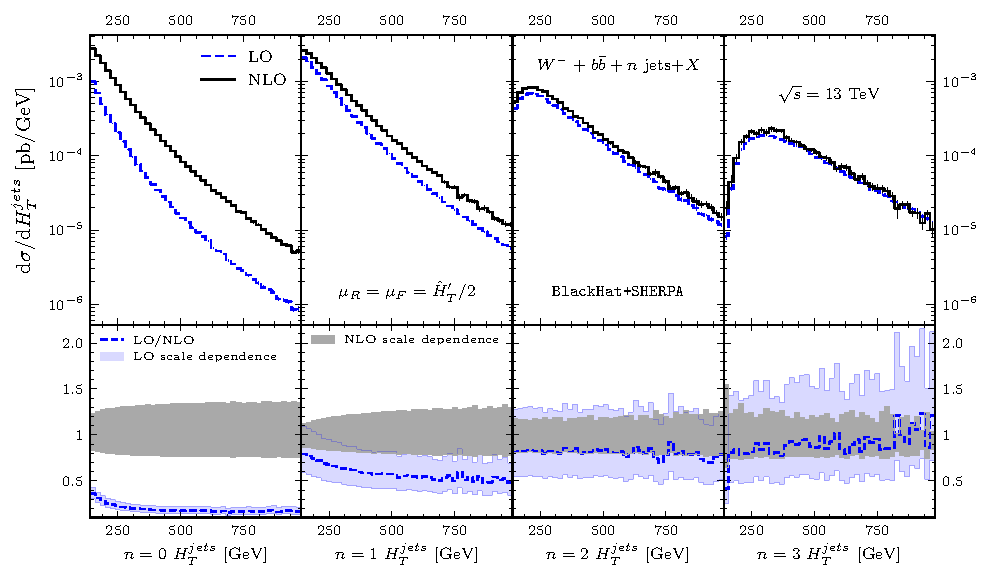
\includegraphics[clip,scale=1.0]{plots/htjets.pdf}
  \caption{Distribution in the total transverse jet energy
    $H_T^{jets}$ of light  and $b$ jets for inclusive \Wbbm$+n$-jet
    production at the LHC with $\sqrt{s}=13$~TeV. Format as in \cref{fig_Wmnjpt}.}
    \label{fig_Wmnjht}
  \end{figure}
%%%%%%%%%%%%%%%%%%%%%%%%%%%%%%%%%%%%%%%

An interesting observable for many scenarios of physics beyond the SM (BSM), as
well as for experimental studies at hadron colliders, is that of the total
hadronic activity in a detector. In \cref{fig_Wmnjht} we show the distribution in
this observable, including all hadronic activity from the light and $b$ jets in
\Wbbm$+0,1,2,3$-jet production. Large and phase-space dependent NLO
corrections appear for \Wbb{} as we would expect from previous discussions.
Interestingly, in \Wbbj{} production a remnant of these large effects appears
in this observable. The corrections are not as large as for the former, but still at
around 1~TeV for $H_T^{jets}$, we see a differential $K$-factor reaching two,
though the shape difference seems to end at about 400~GeV. The
large-multiplicity processes on the other hand show much less
structure, related to the kinematically unconstrained nature of their
LO configurations, which contain any $W$ soft enhancements starting at LO.

%dR first b-jet / charged lepton
%%%%%%%%%%%%% FIGURE %%%%%%%%%%%%%%%%%%
\begin{figure}[ht]
  \centering
  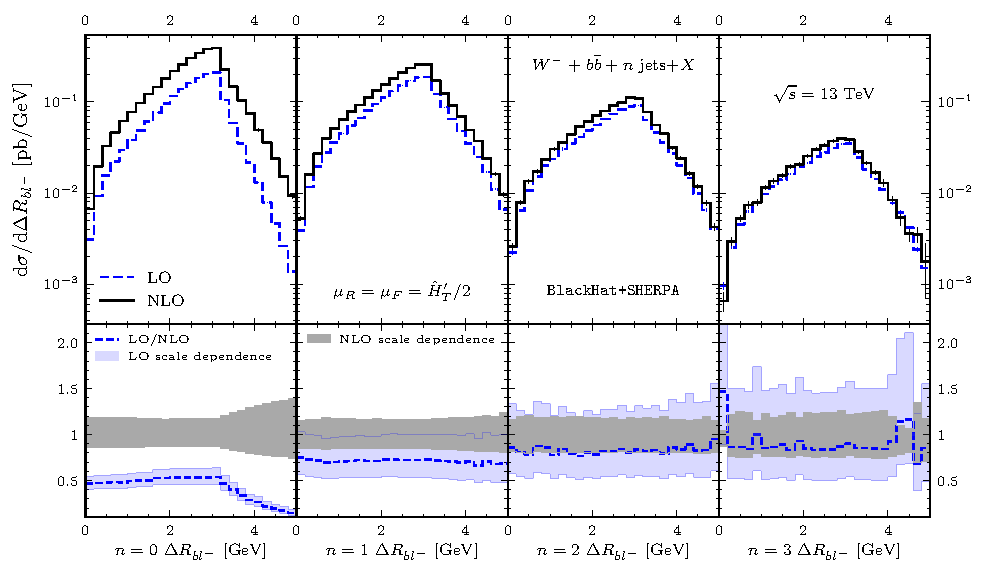
\includegraphics[clip,scale=1.0]{plots/drbl.pdf}
  \caption{Distribution in the $\Delta R_{bl^-}$ separation between the first
  $b$ jet (ordered in $p_T$) and the charged lepton for inclusive \Wbbm$+n$ jets
  production.  Format as in \cref{fig_Wmnjpt}.}
  \label{fig_Wmnjdrbl}
\end{figure}
%%%%%%%%%%%%%%%%%%%%%%%%%%%%%%%%%%%%%%%

Finally, to end this section, we show in \cref{fig_Wmnjdrbl} the distribution
on the $\Delta R$ separation between the first $b$ jet and charged lepton $l^-$. Most
of the angular variables that we have studied are similar to this one, which
shows little structure in the QCD corrections. We only find effects
when a certain kinematic constraint is imposed at LO and released by the corrections,
as it is the case on the left most plots of \cref{fig_Wmnjdrbl}. 
In the case of the $\Delta R_{bl^-}$ at LO in \Wbbm{} production, the parent $W$
and gluon that give rise to the leptons and $b$ jets are produced with $\Delta
\phi$ (the difference in azimuthal angle) equal to $\pi$. Also, the $\Delta \eta$
distribution peaks at around zero and decreases monotonically. The resulting $\Delta R_{bl^-}$ distribution thus has the feature of a sharply decaying
distribution at LO. All
those constrains are lifted by the real corrections and do not appear at all in
\Wbb$+1,2,3$-jet production.


\subsection{Finite $b$ Mass Effects}
\label{sec:bmass}
Mass effects in \Wbb{} have been studied since the early NLO QCD
calculations in ref.~\cite{FebresCordero:2006sj}. They are expected to be small when two
well-defined $b$ jets are considered, and ratios of $m_b^2$ to typical invariants
are small. Nevertheless, their contributions are fundamental when studying
inclusive $b$-jet production at hadron colliders (see for example 
refs.~\cite{Campbell:2008hh,Caola:2011pz}).


%mbb spectrum Wbb & Wbbj ratio massive/massless
%%%%%%%%%%%%% FIGURE %%%%%%%%%%%%%%%%%%
\begin{figure}[ht]
  \centering
  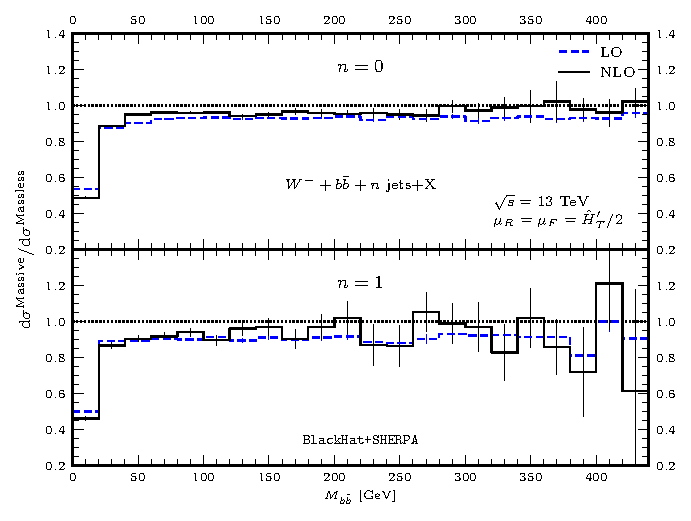
\includegraphics[clip,scale=1.0]{plots/crmbb}
  \caption{Ratio of the invariant mass spectrum of the $b\bar b$ system for 4FNS
    result to the 5FNS ones, for \Wbbm{} (top) and \Wbbm+1-jet (bottom) production.
    The ratios are taken at LO (dashed blue line) and at NLO (solid black line).
    Statistical errors are shown as thin vertical lines. We include a dotted
  horizontal line at a ratio value of 1.}
  \label{fig:ratWmmbb}
\end{figure}
%%%%%%%%%%%%%%%%%%%%%%%%%%%%%%%%%%%%%%%

In order to highlight these effects, in \cref{fig:ratWmmbb} we show the ratio of
a computation performed in the 4FNS consistently keeping the mass of the $b$
quarks, to that of a corresponding massless calculation performed with massless
$b$ quarks in the five-flavor number scheme (5FNS). In the latter we use the
PDFs from CT14~\cite{CT14}, denoted by \texttt{CT14llo} at LO and
\texttt{CT14nlo} at NLO.  We notice that for values of $M_{b\bar b}$ above 50
GeV, the ratios stabilize rapidly at about 0.95 for \Wbb{} production and at
0.9 for \Wbbj{} production, while for values below we have a strong deviation
with the massless calculation more than doubling the massive one. This is to be
expected as phase space constrains the production of massive
$b$ quarks in these regions and also $m_b^2/M_{b\bar{b}}^2$ terms in
the matrix elements can be important.


The mass effects are stable with respect to quantum corrections, as we can
deduce from the similarity of the LO and NLO ratios. We notice that the deviation
from 1 at large $M_{b\bar b}$ is smaller than the scale-dependence bands of the
NLO results, which can be used as a proxy of unaccounted higher-order
corrections. 

The observed behavior is very similar at what was studied in
ref.~\cite{FebresCordero:2006sj} in the case of \Wbb{} production, and here we
extend it to \Wbbj{} production. It is important to mention that although the
computations in \cref{fig:ratWmmbb} are consistent results in the 4FNS and in the
5FNS, they have the same diagrammatic content at Born level, and in
particular there is no $b$-initiated subprocess in the massless
calculation. For
that reason the comparison presented is attributable to $b$-mass effects in the
matrix elements and in phase-space generation, together with the corresponding
differences from the PDFs and their corresponding running couplings. A more
systematic 4FNS vs. 5FNS comparison including \Wbbjj{} and \Wbbjjj{}
production would be more relevant to compare the two schemes, which we leave to
future work. A future study of our results for more inclusive
samples of $W$ production in association with $b$ jets will also be
interesting (in this study we focus in signatures with exactly 2 $b$ jets).



%%%%%%%%%%%%%%%%%%%%%%%%%%%%%%%%%%%%%%%%%%%%


\subsection{Backgrounds to The Associated Production of $H$ and $W$}
\label{sec:hw}

So far all LHC measurements of Higgs-boson properties appear in good agreement
with predictions of the SM 
(see for
example ref.~\cite{Khachatryan:2016vau}). One of
the properties that will be important to constrain further is the coupling strength of the Higgs
boson to $b$ quarks. Given that a Higgs boson with mass $M_h$ around 125 GeV is
supposed to decay more than half of the time into a $b\bar b$ pair, it is of great
importance to constrain the Yukawa coupling $y_b$ and consequently 
learn about the Higgs boson's total decay width.
In the main
production channel of the Higgs, through gluon-gluon fusion, one faces
a large background from pure QCD $b\bar b$ production. Therefore,
considering the associated $Wb\bar b$ production gives an extra handle to
detect the Higgs decaying to $b$ quarks (see the recent measurement by ATLAS in
ref.~\cite{ATLAS:hbb2017}). This of course, as long as the
irreducible backgrounds for \Wbb{} production in the SM can be kept under
control. The predictions provided in this article aim to contribute
to these studies.

Some of the key observables for $HW$ analyses are those associated to the $b\bar
b$ system, in particular $p_T^{b\bar b}$ and $M_{b\bar b}$. When
producing a Higgs, those are associated with the $p_T$ distribution
and the invariant mass of the Higgs. In addition,
distributions that help to characterize the accompanying $W$ boson are important, for
example $p_T^W$. In this section we study those three observables 
with our high-multiplicity results.
 At high energies the presented spectra are
enhanced with resonant top contributions (see for example the recent
study~\cite{Denner:2017kzu}). Nevertheless, in the context of $HW$ production
the focus is on the non-resonant backgrounds. The non-resonant top contributions
are sizable, and can be of similar order to the ones presented here. We leave
studies of non-resonant top contributions to future work.

%pt(bb) 
%%%%%%%%%%%%% FIGURE %%%%%%%%%%%%%%%%%%
\begin{figure}[ht]
  \centering
  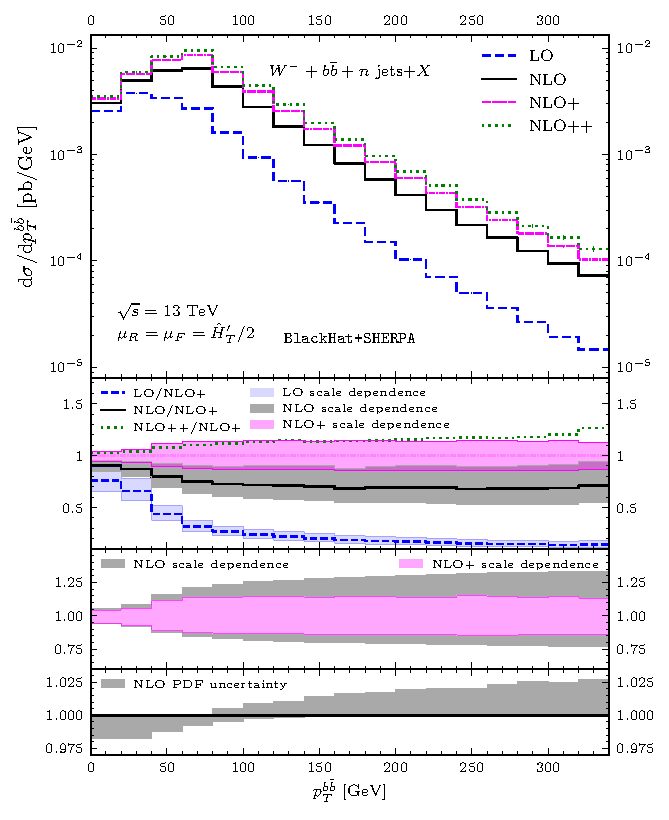
\includegraphics[clip,scale=1]{plots/excl_ptbb_v4}
  \caption{The $p_T$ distribution of the $b\bar{b}$ system in inclusive \Wbbm{} production,
    computed at LO (dashed blue line) and NLO (solid black line) as well as
    by employing the exclusive sums NLO+ (dashed-dot magenta line)
    and NLO++ (dotted green line).
    The second panel shows scale dependence bands normalized by NLO+,
    and in the third panel they are normalized by the corresponding
    central value. The bottom panel shows the associated PDF uncertainties
    normalized to our NLO results.}
  \label{fig_Wmnjptbb}
\end{figure}
%%%%%%%%%%%%%%%%%%%%%%%%%%%%%%%%%%%%%%%

The NLO QCD correction to \Wbb{} production have large contributions associated to
processes with an extra light jet~\cite{Ellis:1998fv,FebresCordero:2006sj,Cordero:2009kv}.
 A way to handle those
contributions was to obtain exclusive results in the number of light
jets~\cite{FebresCordero:2006sj}, which explicitly vetoed
events with extra jets, but that prescription suffers from its sensitivity
to the $p_T^\mathrm{veto}$ cut~\cite{Tackmann:2012bt}. 
In this article we consider a different approach, using the `exclusive sums'
technique~\cite{ESums}.
Instead of imposing a veto cut to stabilize the predictions, this approach
replaces the extra light-jet contributions to generic observables,
which are effectively LO, by their corresponding results including NLO QCD
corrections. In higher-order corrections such contributions are naturally
added. However, as they are hard to obtain, we use the above
approximation and analyze the impact in our predictions.


The `exclusive sums' technique is expected to give improved predictions when
tree-like contribution, with an extra light jet, to NLO corrections are 
large. Notice that in measurements of $W$+light jets some of the predictions
from exclusive sums have been compared to LHC data, see for
example~\cite{Aad:2014qxa,ATLAS:ratio2017}, usually in the context of $W+1$-jet production. By
now those computations are outdated, given the recent NNLO QCD calculation
presented in ref.~\cite{Boughezal:2015dva}. It is important to mention that for the comparison to LHC data the
application of a parton-shower can be studied \cite{Luisoni:2015mpa}, or using a
matched and merged version for example with the MEPS@NLO \cite{Hoeche:2012yf} or FxFx technique \cite{Frederix:2012ps}.


We will focus on predictions for \Wbb$+X$ production. Fixed-order
results for those will be denoted as usual with the labels LO and NLO. The
exclusive sums we employ are defined in Eq.~\eqref{eq:excsums}, for which we
will use the labels NLO+ and NLO++.
We will use the latter only as a proxy for the size of even
higher-order corrections, that is as an estimator of theoretical uncertainty.
Our main predictions will be that of NLO+.

For completeness, to characterize theoretical uncertainties, we will also explore the PDF uncertainty associated to the
observables under consideration, even though 
they turn out to be subleading. In order to estimate the PDF uncertainty we use
the error sets from the pseudo-PDF set
\texttt{PDF4LHC15\_nlo\_nf4\_30}~\cite{Butterworth:2015oua}. 
Given the smallness of the PDF errors compared to
other theoretical uncertainties, we do not go beyond this
restricted error set for our estimations. Other sources of
uncertainties are the values of $m_b$ and $\alps$, but those are expected to
be rather small, e.g.\ when compared to missing higher-order corrections.

%pt(W) 
%%%%%%%%%%%%% FIGURE %%%%%%%%%%%%%%%%%%
\begin{figure}[ht]
  \centering
  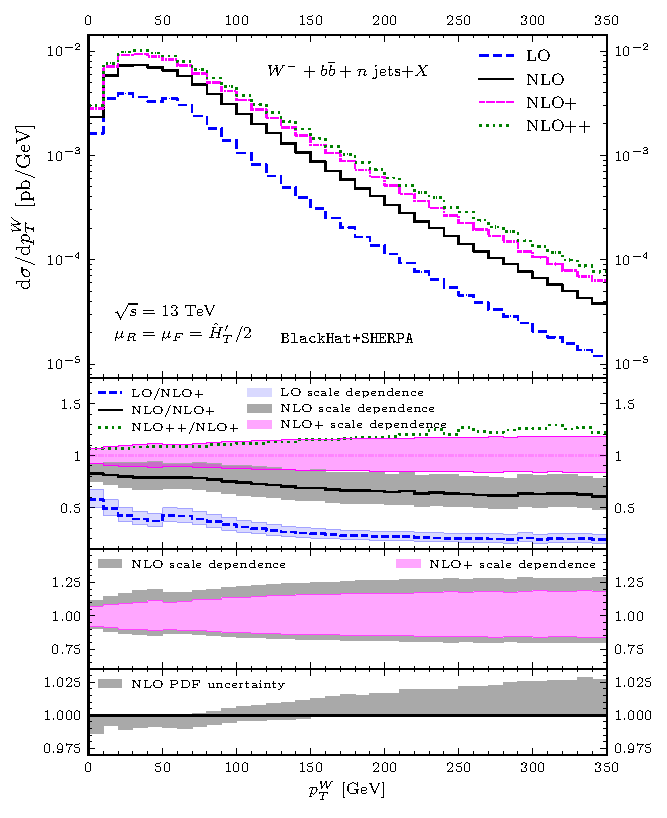
\includegraphics[clip,scale=1]{plots/excl_ptw_v4}
  \caption{The $p_T$ of the $W$ boson in inclusive \Wbbm{} production. Format as in \cref{fig_Wmnjptbb}.}
  \label{fig_Wmnjptw}
\end{figure}
%%%%%%%%%%%%%%%%%%%%%%%%%%%%%%%%%%%%%%%

In \cref{fig_Wmnjptbb}, we show the transverse momentum distribution of
the $b\bar b$ system. In the upper panel, we show all of our predictions, including the central `NLO+' prediction as well as LO, NLO
and NLO++. The second panel shows the corresponding scale-dependence bands at
LO, NLO and NLO+, all normalized by NLO+, as well as the central value for
NLO++. In the third panel we show the scale-dependence bands at
NLO and NLO+, normalized by their corresponding central value. In the bottom panel we show the PDF uncertainties, which are always below
2\% for all the ranges of $p_T^{b\bar b}$ shown (we normalized the PDF
uncertainties by our central NLO result). The scale-dependence bands
of the NLO+ predictions are at the level of 13\%, which is a reduction compared to the 26\%
of the fixed-order NLO result. The LO result gives no adequate
prediction. The NLO and NLO+ bands overlap, though they show a difference in
shape, particularly at low values of $p_T^{b\bar b}$. We find that the
higher-order corrections estimated through scale variations and by the NLO++
results are of the same order of magnitude, at the level of 10\%.

For the $p_T^{b\bar b}$ observable, one obseves the release of
kinematical constraints at NLO (which tights up $p_T^{b\bar b}$ and $p_T^W$).
Since at LO the massive $b$-quark pair
originates in a gluon splitting, the kinematical constraints in \Wbb{} are
similar to those appearing in $V+1$ light jet (see e.g.\ refs.~\cite{BH:W3jPRL,BH:W4j,BH:W5j}). Real-radiation emission relaxes this
constraint and yields large corrections at NLO through a soft enhancement, which
gives rise to a giant $K$-factor~\cite{Rubin:2010xp}. These characteristics of
the NLO results for \Wbb{} production are then expected~\cite{Catani:1997xc} and
require resummation although fixed order corrections are known to improve the
predictions~\cite{Ridder:2015dxa}.


%Mbb 
%%%%%%%%%%%%% FIGURE %%%%%%%%%%%%%%%%%%
\begin{figure}[ht]
  \centering
  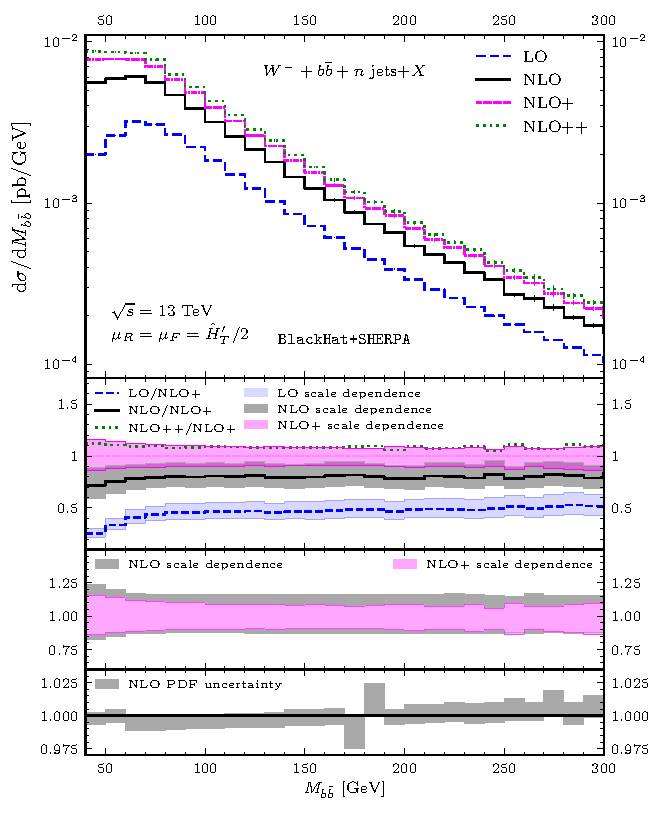
\includegraphics[clip,scale=1]{plots/excl_mbb_v4}
  \caption{The invariant mass of the $b\bar b$ system in inclusive \Wbbm{} production. Format as in \cref{fig_Wmnjptbb}.}
  \label{fig_Wmnjmbb}
\end{figure}
%%%%%%%%%%%%%%%%%%%%%%%%%%%%%%%%%%%%%%%

In \cref{fig_Wmnjptw}, we show in the same manner the distribution in the transverse
momentum of the vector boson $p_T^W$. The results are again similar to what we
encounter for $p_T^{b\bar b}$, with the NLO+ uncertainty estimation marginally
overlapping with the NLO predictions and with its scale sensitivity of the order
of the NLO++ predictions. The estimation of theoretical uncertainties is about 17\% in the
range of $p_T^W$ shown (as compared to the 25\% of the NLO results). Again, the PDF uncertainties are
subleading, appearing at 3\% and below.

Finally in \cref{fig_Wmnjmbb} we show the distributions in the $M_{b\bar b}$
observable, which exhibit similar features to the observables
studied previously in this section. In this case, the uncertainties associated with scale
sensitivity and missing higher-order effects appear at about 10\% or slightly
smaller. The PDF uncertainties are tiny, being at 1\% or smaller. 


